\chapter{Results and Discussion}

\section{Time calibration}
\label{chap:time cal}
In this part a suitable calibration to transform the channel axis to a time axis is determined. In order to collect appropriate measurements for that, the moveable detector is fixed at the minimal distance from the source, an the discriminator threshold is set to a value of 55, so that most $\SI{511}{keV}$ quanta are detected, but any noise is cut off. The manual delay of the TPC is set to $\Delta t = \SI{2}{ns}$ which works as the zero value. Now, the spectrum is measured at multiple manual delay times, from $\Delta t = \SIrange[]{0}{32}{ns}$ with a distance of \SI{4}{ns} each. A measured spectrum can be seen in figure \ref{fig:0nsnofit}.

\begin{figure}[H]
    \centering
    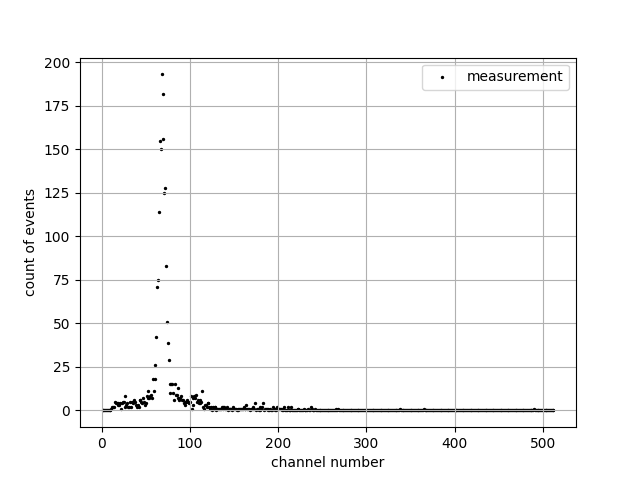
\includegraphics[width=110mm,scale=0.5]{Positronium/include/0nsnofit.png}
    \caption{Measured time sprectum at 0ns manual delay} 
    \label{fig:0nsnofit}
\end{figure}

For each of the time spectra, the peak is fitted to a gaussian distribution to find out its channel number. For each fit an uncertainty of 3 is assumed on the channel, the figures of this can be found in the appendix chapter \ref{chap:appendix time calibration}. The resulting peak channel numbers can be found in table \ref{tab:mu table}.\\
\begin{table}[]
    \centering
    \caption{fit results of all measured time spectra}
    \begin{tabular}{cccccccccc}
      $\Delta t$ in ns & 0 & 4 & 8 & 12 & 16 &20 & 24 & 28 & 32 \\
    \hline
    $\mu$ & 68.41 & 117.09 & 168.10 & 218.18 & 269.13
& 319.52 &371.52 & 422.00 & 470.22\\
    $\sigma_\mu$ &0.03& 0.05 &0.05 &0.06& 0.06& 0.07&
 0.05& 0.05 &0.04 \\\hline
    \end{tabular}
    \label{tab:mu table}
\end{table}{}

\\
\\The set of peak channel numbers can then be linearly fitted to the manual delay time with this function: 
$$ t = a\cdot\mu +b$$
where $\mu$ is the peak channel number and $a,b$ parameters to be determined. \\The fit is shown in figure \ref{fig:timecalfit}. The uncertainty on the peak channel numbers ranges from $\SIrange{0.03}{0.07}{}$, which is very small compared to their value, so they are not visible in the figure.

The results of the fit can be seen in table \ref{tab:timecalfit}.

\begin{figure}[]
    \centering
    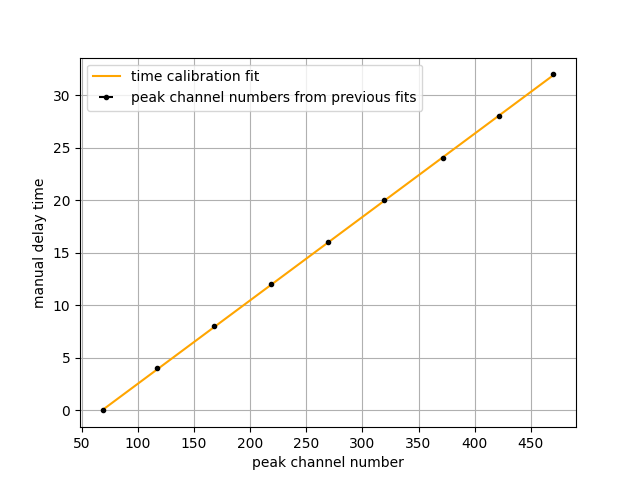
\includegraphics[width=110mm,scale=0.5]{Positronium/include/timecalfit.png}
    \caption{Manual delay time fitted to peak channel number} 
    \label{fig:timecalfit}
\end{figure}

\begin{table}[]
    \centering
    \caption{Results of the time calibration fit}
    \begin{tabular}{cc c}
        parameter & a & b \\ \hline
        estimate & 0.07934 & -5.38240 \\
        uncertainty & 0.0001  &0.03369\\
        \hline
    \end{tabular}
    
    \label{tab:timecalfit}
\end{table}
To determine the time resolution of the TPC, it is necessary to determine the full width half  maximum (FWHM) of each measured spectrum. However, a gaussian distribution was already fitted to each measured spectrum, so the FWHM is given by 
$$FWHM = 2 \cdot \sqrt{2\cdot\ln{2}} \cdot \sigma$$
with $\sigma$ being the standard deviation of the fitted gaussian. It's uncertainty is determined trough gaussian error propagation: 
$$\sigma_{FWHM} = \sqrt{(2 \cdot \sqrt{2\cdot\ln{2}} \cdot \sigma_\sigma)^2}$$
with $\sigma_\sigma$ being the uncertainty of the standard deviation of the fitted gaussian.
The time resolution can then be determined by the following:
$$\delta t = FWHM \cdot a$$ and its uncertainty $$\sigma_{\delta t} = \sqrt{(a \cdot\sigma_{FWHM})^2 + (FWHM \cdot \sigma_a)^2}$$
with a being the parameter determined earlier.
The results are displayed in table \ref{tab:time res}. From this, a weighted mean can be calculated, using the inverse of the square uncertainties as weights. 
The weighted mean is given by 
$$\frac{\sum_i{\delta t_i \cdot p_i}}{\sum_i{p_i}}$$
and it's uncertainty
$$\frac{\sqrt{\sum_i{(\delta t_i \cdot p_i)}^2}}{\sum_i{p_i}^2}$$
with $p$ being the inverse of the squared uncertainty $\sigma_{\delta t}$.
With this, the weighted mean of the time resolution is given by: 
$$\delta t = 0.6937 \pm 0.2562$$
These results convey that the current time resolution of the TPC is too high to distinguish the para-positronium and the free positron-electron annihilation, so they're treated as having the same lifetime going further.  

\begin{table}[]
    \centering
    \caption{Time resolution calculation results}
    \begin{tabular}{cccccccccc}
         $\Delta t$ in ns & 0 & 4 & 8 & 12 & 16 &20 & 24 & 28 & 32 \\\hline 
         FWHM & 8.951& 8.640& 8.615 &8.626& 8.849& 9.138& 8.664& 9.088 &8.261 \\
         $\sigma_{FWHM}$ & 0.082 &0.136& 0.122& 0.164& 0.145& 0.167& 0.121& 0.126 &0.100 \\
         $\delta t$ &0.7102 &0.6856 &0.6835 &0.6844& 0.7022 &0.72512
 &0.6874 &0.7211& 0.6555 \\
         $\sigma_{\delta t}$ &0.0066 & 0.0108& 0.0097& 0.0130 &0.0115& 0.01333&
 0.0097& 0.0101 &0.0080 \\\hline
    \end{tabular}
    \label{tab:time res}
\end{table}

\section{Lifetime of the Positronium}

To determine the lifetime of the positronium, a spectrum of its decay has to be measured over a long period of time, in this case roughly an hour. The discriminator is setup in a way that the $\SI{1.276}{MeV} \gamma$-quantum acts a a start signal, and any of the $\SI{511}{keV}$-quanta, even those which lost energy during pick-off processes act as the stop signal for each measurement point, just the noise is cut off from the spectrum. 
The channel axis of the recorded spectrum is transformed to a time axis, as described in chapter \ref{chap:time cal}. Then, the spectrum below $t = \SI{0}{ns}$ is cut off. The resulting spectrum can be fitted to the function: 
$$\mathrm{counts} = A\cdot\exp{-\frac{t}{\tau_1}}+ B\cdot\exp{-\frac{t}{\tau_2}} + C $$
with $A,B$ as amplitudes which are not of further interest, $C$ the off, which is also not of further interest and $\tau_1, \tau_2$ as the lifetimes of the positronium.
The function is fitted to the spectrum using kafe2, which can handle both the uncertainties in counts and time. An uncertainty of 4 is assumed on the counts, while the uncertainty on the time is linearly propagated using the python uncertainties package. With both uncertainties determined, kafe2 delivers the results seen in figure \ref{fig:lifetime} and table \ref{tab:lifetime}. As seen in the figure, most of the measurements are within the 1-$\sigma$ band, however there are suspiciously many outside the 1-$\sigma$ band, which hints towards underestimated uncertainties. Which uncertainties might be too low could not be determined.\\
We recognize the lifetime $\tau_1$ as the lifetime of the para-positronium and the lifetime of the free positron under electron-positron annihilation. In our setup, these cannot be distinguished, for reasons already discussed at the end of chapter \ref{chap:time cal}. We recognize the lifetime $\tau_2$ as the lifetime of the ortho-positron.
Comparing these values to literature values\cite{BlueBook}, $\tau_{para} = \SI{0.12}{ns}$ , $\tau_{ortho} = \SIrange[]{2}{4}{ns}$, $\tau_{free} = \SI{0.5}{ns}$, one can see that the lifetime of ortho-positron is within the calculated uncertainty, while both the free positron-electron annihalation and para-positron annihalation is outside the calculated uncertainty. This, again, hints towards underestimated uncertainties. The skew of $\tau_1$ towards the lifetime of the free positron is shaped by the relative prevalence of the decay: In polymers, the free positron decay makes up about 60-80\% of all decays, while the para-positronium decay only contributes about 10\%.



\begin{figure}[]
    \centering
    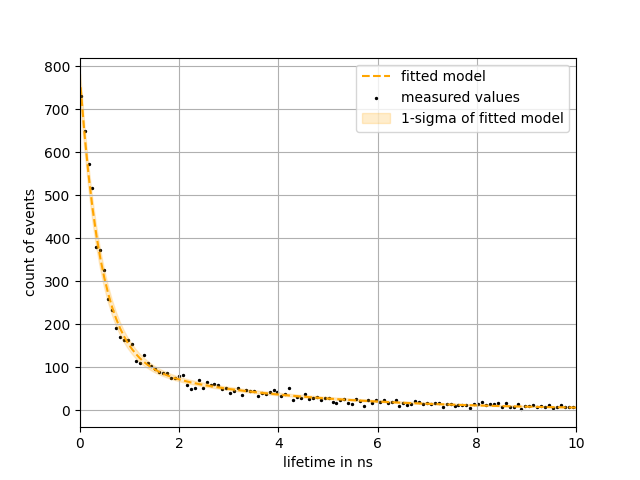
\includegraphics[width=110mm,scale=0.5]{Positronium/include/lifetimefit.png}
    \caption{Lifetime spectrum fit graphical result} 
    \label{fig:lifetime}
\end{figure}

\begin{table}[H]
    \centering
    \caption{Lifetime spectrum fit numerical results}
    \begin{tabular}{cccccc}
         parameter & A& B & $\tau_1$ & $\tau_2$ & C\\ \hline
         estimate & 653 & 118.9 & 0.424 & 3.4 & 0.19\\
         uncertainty & 25 & 4.4& 0.015& 0.11& 0.26 \\\hline \\
    \end{tabular}
    \label{tab:lifetime }
\end{table}

\section{Speed of Light}
As the last part of this experiment, the speed of light is determined. 7 spectra of different detector distances are recorded. The increased distance leads to a lower signal rate, but also a shift of the spectrum peak to higher channel numbers. Using the results from chapter \ref{chap:time cal}, the channel number-axis is transformed to a time axis. To determine the time difference between each spectrum, the measured spectrum peaks are fitted to a gaussian distribution. The fits can be found in the appendix chapter \ref{}